% Appendix C -- the final prompt position.
\section{The geometry at the final position, in full}
\label{app:geometry}

Table~\ref{tab:behaviour} says the effect is content: a document that is present
but wrong is worth nothing. The internal picture at the last prompt position says
the opposite, and it says so exactly where the document is being read. The cosine
between the displacement caused by the skill and the displacement caused by an
unrelated document of similar length is $0.93$ at layer 0, $0.9475$ at layer 4
and $0.91$ at layer 10 on the synthetic control, falling to $0.35$--$0.41$ only
from layer 18, i.e.\ after the model has stopped reading (\S\ref{sec:where}). On
a second family the same comparison at layer 10 gives $0.9716$ between two
mutually exclusive skills against $0.9445$/$0.9555$ between each of them and an
unrelated document---a gap of $0.016$--$0.027$ with bootstrap intervals of width
$0.001$, so it is real and it is negligible.

Read alone, that says the injection is not content-specific. Under
Eq.~\ref{eq:decomp} it says something narrower and correct: over the first half
of the network $\|\dvec\|$ is only $0.38$--$0.45$ of $\|\tvec\|$, so most of what
a cosine between $h_{\text{skill}}$ and $h_{\text{wrong}}$ measures is shared,
and the interesting quantity is the part that is not. Three facts follow, all in
Figure~\ref{fig:decomp} with the numbers in Appendix~\ref{app:tables}. The
content component is a minority of the displacement wherever the document is
being read---under half of $\|\tvec\|$ through layer 14. Through layer 16
$\|\gvec\|$ actually exceeds $\|\tvec\|$: the \emph{wrong} document moves the
state further than the right one, and the two components partly cancel, which is
why the ratio recovers deeper without $\gvec$ shrinking. And two items' content
vectors are far more aligned when they use the same row of the conversion table
than when they do not, so whatever $\dvec$ encodes is about the document's
content rather than about the item.



None of this is causal evidence, and the rest of the paper is about why it
should not be read as any. A displacement can be large and do nothing; a
direction can differ systematically between documents and carry none of its
effect (\S\ref{sec:whose}). We use the geometry only to say which quantity is worth
intervening on, and then intervene.


\subsection{The decomposition and the answer-length ladder, in full}
\label{app:onepos}

We add each component back to the no-document state at the last prompt position
and let the forward pass continue, $h' = h_{\text{no}} + \alpha v$ for
$v \in \{\dvec_i, \gvec_i, \tvec_i, \bar{\dvec}, \dvec_j\}$, against an upper
reference that replaces the state outright with $h_{\text{skill}}$. The
protocol needs a task with an exact zero floor and a matched negative control,
so it is established on the synthetic tier and then carried to the clinical one;
Appendix~\ref{app:decomp} gives the full sweep, and this is the only place in
the paper where the synthetic material carries an argument of its own.

Three results, and the third is the one the rest of the paper uses.
\textbf{The presence component repairs nothing but is not inert}: injected
alone it takes the rescued cell to $0.098$, and putting the wrong document in
the prompt also gives $0.098$---it faithfully reproduces the behaviour of having
\emph{a} document, which is worse than having none. \textbf{The content
component repairs most of the cell}, $0.805$ against an upper reference of
$1.000$, having been dismissed by every geometric measurement as a small
residual. \textbf{The patch reproduces the document's whole behavioural
signature}: across the four cells, replacing the position with
$h_{\text{skill}}$ gives $1.000 / 0.000 / 1.000 / 0.000$ and adding $\dvec_i$
gives $0.805 / 0.075 / 1.000 / 0.186$---the same signature, attenuated. A patch
that only ever helped would be consistent with a generic ``try harder'' effect;
one that also breaks exactly the items the document breaks is carrying the
document's decision.

\paragraph{Which control you subtract chooses what you measure.} $\dvec$ is
defined against a control document, and the choice is a measurement decision
rather than a detail. Against an \emph{unrelated} document of the same length it
is topic, procedure and numbers together and repairs $0.805$ of the rescued
cell; against the \emph{same} document with every number replaced it is the
numbers alone and repairs $0.171$--$0.256$ (layers 21--27); against the same
document with its sentences shuffled, $0.171$--$0.280$. The three differ by a
factor of three to four, so a paper
that reports ``the content component'' without naming its control has not
specified the quantity. Appendix~\ref{app:controls} gives the full comparison.
\subsection{What a single position can carry is the answer, not the content}


Single-position patching is the standard move in this literature, and
Table~\ref{tab:causal} is a multiple-choice result, so it is worth asking what
that one position is carrying. The same items exist in a free-form numeric form,
where the answer is a number the model must compute rather than an option it
must select; there the skill is worth $0.006 \to 0.332$ and the rescued cell
has $119$ of the $358$ items.

Two things change and one does not. The ceiling collapses: through layer 22 no
condition exceeds $0.008$, including replacing the position outright with the
true skill state, and the best any single-position intervention achieves is
$0.235$, at layer 30. What does not change is the ordering---the content
component recovers $0.210$ and the presence component $0.008$---so the
conclusion of \S\ref{sec:decomp} survives the format while the magnitude does
not (full sweep in Appendix~\ref{app:tables}).

\paragraph{It is the format, not the model.} The identical sweep on the
\emph{same model and the same $358$ items} in multiple-choice form (Qwen3-8B,
$n_R=94$) recovers $0.957$ at layer 26 and $1.000$ at layers 29, 30 and 35.
Same model, same items, same intervention, same layers: $1.000$ when the answer
is one option letter, $0.235$ when it is a number the model has to produce.

The reason is mechanical and can be counted. The gold answers run one to five
tokens under this tokenizer and $341$ of the $358$ use two to four. A patch at
one prompt position can fix at most the first generated token; the rest are
produced in a context that still does not contain the conversion table.
Multiple choice compresses the answer to exactly one token---which is exactly
the unit a single-position patch transports. Patching the last $k$ positions
instead of one does \emph{not} lift the ceiling in proportion: $k=1,4,16$
recover $0.235$, $0.261$ and $0.403$, and $k=32,48,61$ recover $0.403$, $0.395$
and $0.370$, so sixteen positions carry about half of what the document carries,
four---the chat suffix---carry nothing extra, and everything past sixteen
carries nothing at all.

\paragraph{On third-party skills the same probe reads nothing.} There,
replacing the final prompt position with the with-skill state repairs at most 3
of 18 rescued items (layer 10) and 0--1 from layer 14 on and transplanting the question span---50 to 1697 positions, into a
length-matched receiver---repairs nothing beyond the receiver's own baseline at
any of seven layers (Table~\ref{tab:realspan}), with the self-transplant arm on
that baseline to the item, so the instrument is live and the null is real.
\S\ref{sec:battery} shows what does work on the same material.

\paragraph{Answer length is the cause, and that is a controlled comparison.}
The step from the synthetic tier to the clinical one changes the skill, the
task, the prompt length and the fraction of it a patch covers, so it cannot on
its own identify what makes the injection fail. We therefore made answer length
the only thing that moves: the \emph{same} 80 synthetic items, the same model,
the same document, prompted to reason step by step and give the answer on a
final \texttt{ANSWER:} line. In that format the skill is worth $0.000 \to
1.000$---every item is rescued, $F=K=B=0$---so there is more effect to recover
than in either other format, and the rescued cell is the whole item set.

The single-position patch recovers $\mathbf{0.000}$ of it
(\S\ref{sec:onepos}), as do $\dvec$ and $\gvec$. The last-layer
instrument check passes on 10 of 10 items in the same run.





\textbf{The range over which ``a skill's effect is carried by a vector'' is true
is the range over which the answer is short}---and the clinical result is then
not a property of that material but an instance of this.

\paragraph{It is a ceiling, and more positions do not raise it.} Patching one
position is a choice, not a measurement, so we repeated the sweep patching the
last $k$ prompt positions for $k \in \{1,4,16,32,48,61\}$, every one of the
$36$ layers. The no-document prompt is $61$--$63$ tokens, so $k=61$ writes all
of it and the ladder has no further rung. Recovery on the rescued cell, at each
$k$'s best layer, is $0.235$, $0.261$, $0.403$, $0.403$, $0.395$ and $0.370$,
and $0.403$ is also the largest value over every $k$ and every layer. Four
positions buy nothing---the last four tokens are the chat suffix---sixteen,
which reach back into the question, roughly double the recovery, and past
sixteen nothing is bought: at $k=32$ the items answered correctly are
item-for-item those answered correctly at $k=16$, with no discordant pair, and
at $k=61$ four are lost and none gained (exact McNemar $p=0.125$). We expected
the ladder to keep climbing and registered that prediction before the larger
$k$ ran; it does not climb.

The ceiling is therefore not a budget, and it is not an artefact of writing a
long prompt's states into a short one: the identical probe, receiver and donor
recover $1.000$ on the rescued cell of the multiple-choice format, where the
answer is one token at one position. What separates $0.403$ from $1.000$ is the
answer format.

It is \emph{not} explained by the patched positions being ones the document
does not occupy. On this same free-form material the document's own $688$
positions do no better: they recover $0.408$ at layer $0$, which is close to
putting the document back, and then at most $0.17$ from layer $3$ and nothing
from layer $15$ (Table~\ref{tab:windows2}), below what the last sixteen
positions reach. In free-form no channel on this task exceeds about $0.41$ at
any layer, so the ceiling is a property of the answer format rather than of
which positions are written. The comparison that does isolate position is on
the clinical material, where receiver, items and layer are held fixed: the
document's own span recovers $0.89$ and up to $256$ positions after it recover
$0.05$ (\S\ref{sec:decomp}).

One thing this ladder does not separate is the receiver. It patches into the
\emph{no-document} prompt, while span injection patches into a length-matched
\emph{wrong-document} one, so a receiver effect is not excluded here. Where we
have measured it---the same decomposition at the final position on the
synthetic multiple-choice task---the wrong-document receiver is never worse
than the no-document one and is better in the middle layers
(Table~\ref{tab:causal}), so it would move the ceiling the wrong way; but we
have not run it in free-form. We therefore read the low ceiling as a scope
condition on single-position and short-suffix patching under a multi-token
answer format, rather than as a negative result about $\dvec$. In a multiple-choice
item the answer \emph{is} one token at one position, so a patch that transports
the model's decision transports the whole task and looks like it transported the
document. What the final prompt position holds by layer 21 is the model's
\emph{answer}, not the document's content---consistent with the knockout result
that reading the document is finished by that layer (\S\ref{sec:where}).
\subsection{The decomposition on the synthetic tier, in full}
\label{app:decomp}

\paragraph{The geometry at that position says the opposite of the behaviour.}
Appendix~\ref{app:geometry} gives that measurement and why it cannot settle the
question on its own. We use geometry only to choose what to intervene on, and
then intervene.


We add each component back to the no-document state at the last prompt position
and let the forward pass continue: $h' = h_{\text{no}} + \alpha v$ for
$v \in \{\dvec_i, \gvec_i, \tvec_i, \bar{\dvec}, \dvec_j\}$. The upper reference
is replacing the state outright with $h_{\text{skill}}$; the lower reference is
no intervention.




Figure~\ref{fig:causal} is the causal counterpart of that geometry (numbers in
Table~\ref{tab:causal}, Appendix~\ref{app:tables}). Four of its curves are worth
reading separately.

\textbf{The presence component repairs nothing}---$0.098$, eight items of 82, at
every layer past 20, and $0.00$--$0.02$ before. It is not inert noise: injected
on its own it takes whole-set accuracy from the no-document baseline of $0.180$
to $0.151$, which is the accuracy of actually putting the wrong document in the
prompt. On the rescued cell it gives $0.098$, and the wrong document in context
also gives $0.098$. It faithfully reproduces the behaviour of having a document
present, and that behaviour is worse than having none.

\textbf{The content component repairs most of the cell}---$0.805$ at layer 26
against an upper reference of $1.000$, having been dismissed by every geometric
measurement in \S\ref{app:geometry} as a small residual.

\textbf{At one patched position it is under-scaled, not incomplete.} The
dose-response is monotone and steep---$\alpha=0.5,1,2$ give $0.31$, $0.81$,
$0.98$---so the missing $0.19$ at $\alpha=1$ is a magnitude deficit along a
correct direction, which is expected: $h_{\text{wrong}} + \dvec_i$ is exactly
$h_{\text{skill}}$, while adding $\dvec_i$ to $h_{\text{no}}$ lands elsewhere.
It does not generalise to more positions: at $k=16$ in free-form the dose is
flat between $\alpha=1$ and $2$ ($0.232$, $0.268$) and never approaches the full
replacement's $0.554$. The two components are additive by construction and not
additive in effect. What survives every configuration is the asymmetry: $\gvec$
alone is inert at every $k$, layer and $\alpha$.

\textbf{The receiver does not matter, and a single shared vector is not enough.}
Injecting $h_{\text{skill}}$ into the prompt that already holds the \emph{wrong}
document gives $0.979$--$1.000$, the same as into a prompt with no document---%
whatever the surrounding 700 tokens contribute, the final position does not need
it. But $\bar{\dvec}$, one vector for the whole item set, which is what ``a
reusable skill vector'' would mean, recovers $0.049$--$0.122$ from layer 21
against $0.500$--$0.805$ for the item's own. Splitting $\dvec_i$ along
$u=\bar{\dvec}/\|\bar{\dvec}\|$ and orthogonal to it and injecting each half
separates them and reverses the answer at layer 21: past it the parallel half
carries $\approx 0.9$ of the norm and $0.05$ of the effect while the orthogonal
half carries $0.44$ of the norm and $0.60$ of the $0.81$; before it the two swap,
inside the band \S\ref{sec:traps} independently identifies as one where the
forward pass is disturbed.

\paragraph{The patch reproduces the document's whole behavioural signature, not
just its successes.} Across all four cells, replacing the final position with
$h_{\text{skill}}$ gives $1.000 / 0.000 / 1.000 / 0.000$ on
rescued / persistent / kept / broken at layer 26 on the 1.7B, and
$1.000 / 0.024 / 1.000 / 0.000$ at layer 30 on the 8B---cell by cell, what the
document itself does by the definition of the cells. It reproduces the skill's
failures and its damage as faithfully as its repairs. Adding $\dvec_i$ gives
$0.805 / 0.075 / 1.000 / 0.186$ and $0.864 / 0.024 / 1.000 / 0.077$: the same
signature, attenuated. A patch that only ever helped would be consistent with a
generic ``try harder'' effect; one that also breaks exactly the items the
document breaks is carrying the document's decision. The presence component
passes the matching test against \emph{its} document: $h_{\text{no}}+\gvec$
scores $0.098$ on the rescued cell where the wrong document in context scores
$0.098$ (1.7B), and $0.250$ where it scores $0.250$ (8B), across four different
control documents (Appendix~\ref{app:controls}).




\begin{figure*}[tbp]
\centering
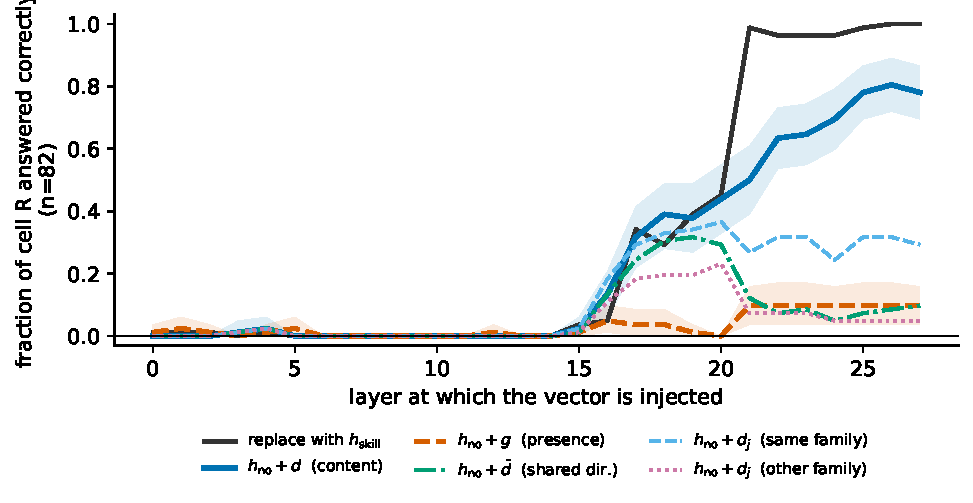
\includegraphics[width=0.86\textwidth]{fig-causal-tierA.pdf}
\caption{What each injected component repairs, on the cell the document
rescues. Shaded bands are bootstrap 95\% CIs for the two conditions the argument
rests on. $h_{\text{no}}+\tvec$ is omitted because it equals $h_{\text{skill}}$
identically and its curve lies under the black one---we run it, and it agrees
item by item. Synthetic control, multiple choice, Qwen3-1.7B, fp32, $n=358$,
rescued cell $n_R=82$.}
\label{fig:causal}
\end{figure*}

\begin{figure*}[tbp]
\centering
\begin{tikzpicture}[>=Stealth, every node/.style={font=\small}]
  \coordinate (no)  at (0,0);
  \coordinate (fil) at (6.24,0);
  \coordinate (yes) at (24.7:5.76);
  \draw[->, very thick, black!50] (no) -- (fil);
  \node[black!50, below=3pt] at ($ (no)!0.5!(fil) $) {$\gvec$\, presence};
  \draw[->, very thick, blue!65!black] (fil) -- (yes);
  \node[blue!65!black, left=3pt] at ($ (fil)!0.5!(yes) $) {$\dvec$\, content};
  \draw[->, thick, dashed, black!35] (no) -- (yes);
  \node[black!40, above left=-1pt and 6pt] at ($ (no)!0.55!(yes) $)
       {$\tvec$\, total};
  \fill (no) circle (2pt) node[left=2pt] {$h_{\text{no}}$};
  \fill (fil) circle (2pt) node[below=4pt] {$h_{\text{wrong}}$};
  \fill (yes) circle (2pt) node[above=3pt] {$h_{\text{skill}}$};
  \node[align=left, font=\footnotesize, black!55, anchor=west] at (7.4,-0.45)
    {larger than $\tvec$ through layer 16;\\
     repairs \textbf{0} items at every layer};
  \node[align=left, font=\footnotesize, blue!65!black, anchor=west] at (7.4,1.55)
    {effective rank 3--8 of 2048;\\
     repairs \textbf{0.77} of the rescued items};
\end{tikzpicture}
\caption{The decomposition, drawn to scale at layer 10 of the synthetic control
($\|\gvec\|=39.0$, $\|\dvec\|=16.3$, $\|\tvec\|=36.0$). A document of the right
length and the wrong content already moves the final prompt position most of the
way---in fact slightly further than the real skill does, which is why the
content arrow points partly back. Everything this paper is about is the short
blue arrow.}
\label{fig:schematic}
\end{figure*}

\begin{table*}[tbp]
\caption{The same items under two answer formats. Top: the effect itself. In
multiple choice the small model shows a $+11$pp skill effect over an $0.18$
floor; in free-form it shows nothing at all, over a floor of exactly zero, and
the effect appears only at 8B. Top block and the multiple-choice column of the
bottom block are the $358$-item reruns; the free-form control column is the
earlier $120$-item sample, which has not been rerun with the corrupted and
scrambled documents. Bottom: the same four documents under both formats, where
``share'' is $(\text{acc}-\text{none})/(\text{gold}-\text{none})$. Destroying
every number in the document keeps just over half of the effect in multiple
choice and none of it in free-form.}
\label{tab:format}
\centering
\small
\begin{tabular}{llcccc}
\toprule
model & format & no document & wrong document & gold skill & effect \\
\midrule
Qwen3-1.7B & multiple choice & 0.179 & 0.151 & 0.288 & $+10.9$pp \\
Qwen3-1.7B & free-form       & \textbf{0.000} & --- & \textbf{0.000} & $\mathbf{0}$ \\
Qwen3-8B   & multiple choice & 0.274 & 0.249 & 0.425 & $+15.1$pp \\
Qwen3-8B   & free-form       & \textbf{0.006} & \textbf{0.006} & \textbf{0.332} & $\mathbf{+32.6}$\textbf{pp} \\
\midrule
\multicolumn{2}{l}{document in context} & \multicolumn{2}{c}{multiple choice (1.7B)} & \multicolumn{2}{c}{free-form (8B)} \\
\multicolumn{2}{l}{} & acc & share & acc & share \\
\midrule
\multicolumn{2}{l}{none}                        & 0.179 & --- & 0.000 & --- \\
\multicolumn{2}{l}{same document, \emph{factors} replaced} & 0.237 & 0.54 & \textbf{0.000} & \textbf{0.00} \\
\multicolumn{2}{l}{same document, \emph{lines} scrambled}  & 0.268 & 0.82 & 0.325 & 0.70 \\
\multicolumn{2}{l}{gold skill}                  & 0.288 & 1.00 & 0.467 & 1.00 \\
\bottomrule
\end{tabular}
\end{table*}

\begin{figure*}[tbp]
\centering
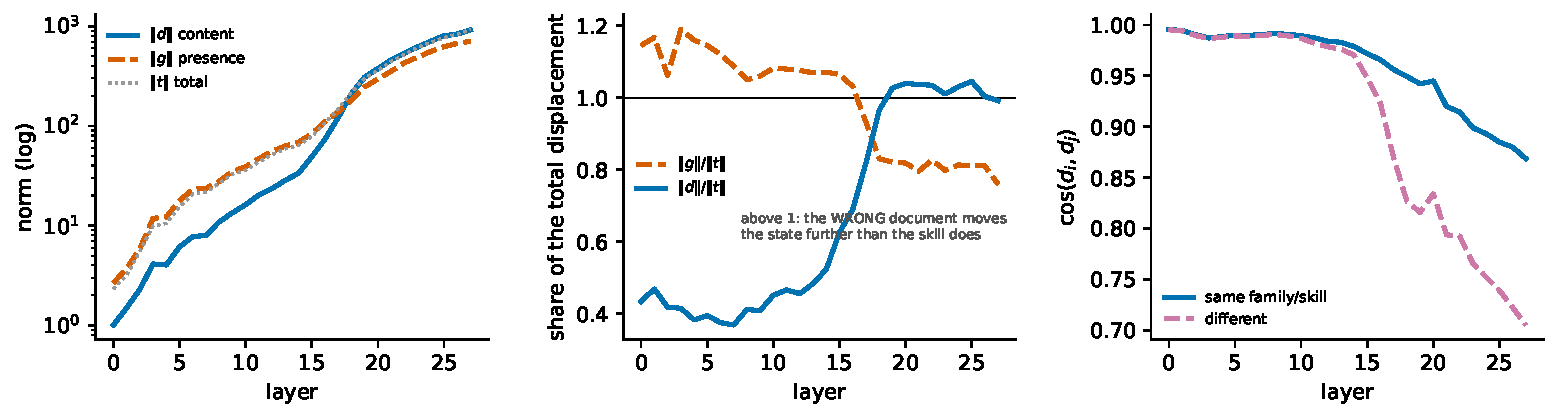
\includegraphics[width=\textwidth]{fig-decomp-tierA.pdf}
\caption{The decomposition across depth, synthetic control, Qwen3-1.7B, fp32,
$n=358$. Left: the three norms. Middle: each component as a share of the total
displacement; above $1$ the wrong document moves the state further than the skill
does, which is the case until layer 17. Right: how aligned two items' content
vectors are, split by whether they use the same row of the conversion table.}
\label{fig:decomp}
\end{figure*}

\begin{figure*}[tbp]
\centering
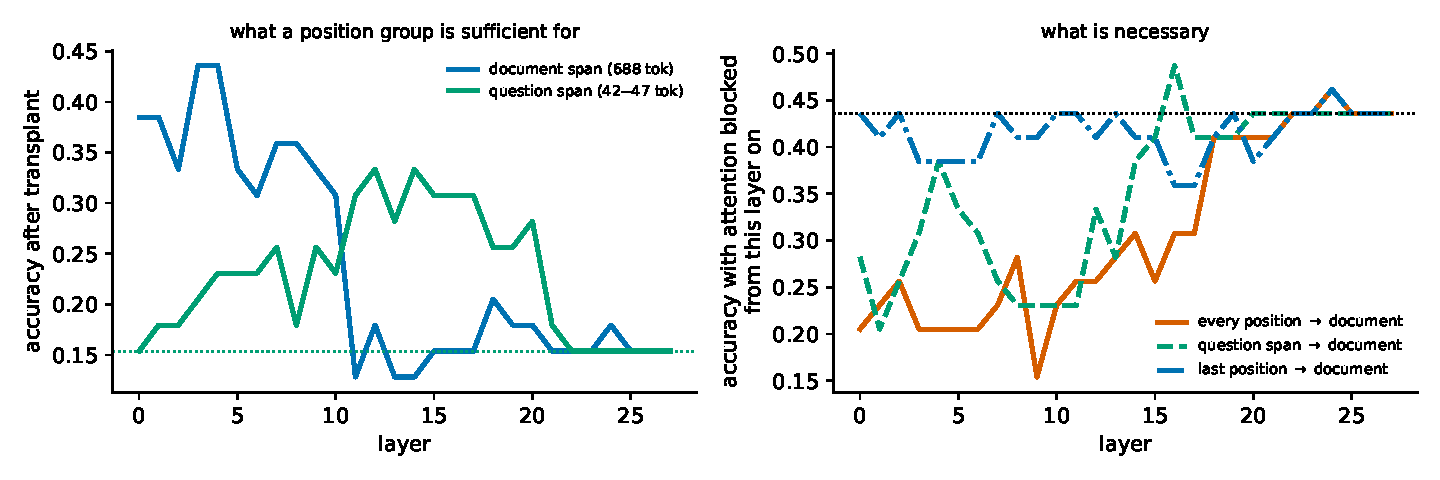
\includegraphics[width=\textwidth]{fig-windows-tierA.pdf}
\caption{Left: what each position group is sufficient for, as a function of the
layer at which its states are transplanted; dotted lines are each channel's own
receiver baseline. Right: what is necessary---accuracy when attention to the
document is masked from the given layer to the end, cumulatively; the dotted
line is the unmasked baseline. Synthetic control, multiple choice, Qwen3-1.7B,
$n=39$.}
\label{fig:windows}
\end{figure*}

\begin{table*}[tbp]
\caption{Peak accuracy of each transplant channel, by model and answer format.
``Donor'' is the with-skill forward and ``receiver'' the prompt being patched
into; the two span channels patch into a length-matched filler-substituted
prompt, the final-position channel into the no-document prompt, which is why
their baselines differ. The final-position rows are the $358$-item reruns; the
two span channels are the earlier $39$-item transplant runs, which were not
rerun. Peaks in \textbf{bold} where the channel recovers most
of the donor.}
\label{tab:windows2}
\centering
\small
\begin{tabular}{llccc}
\toprule
channel & configuration & recv. & peak (layers) & donor \\
\midrule
\multirow{3}{*}{document span (688 tok)}
 & 1.7B, multiple choice & 0.154 & \textbf{0.436} (3--4) & 0.436 \\
 & 8B, multiple choice   & 0.233 & \textbf{0.575} (0--6) & 0.550 \\
 & 8B, free-form         & 0.008 & 0.408 (0 only)        & 0.467 \\
\midrule
\multirow{3}{*}{question span (26--50 tok)\hspace{-2mm}}
 & 1.7B, multiple choice & 0.154 & 0.333 (12--14)        & 0.436 \\
 & 8B, multiple choice   & 0.233 & \textbf{0.517} (21)   & 0.550 \\
 & 8B, free-form         & 0.008 & 0.025 (any, i.e.\ none) & 0.467 \\
\midrule
\multirow{3}{*}{final position(s)}
 & 1.7B, MC, rescued cell & 0.000 & \textbf{1.000} (26--27) & 1.000 \\
 & 8B, MC, rescued cell   & 0.000 & \textbf{1.000} (29--35) & 1.000 \\
 & 8B, free-form, rescued cell & 0.000 & 0.235 ($k$=1), 0.403 ($k$=16) & 1.000 \\
\bottomrule
\end{tabular}
\end{table*}

\begin{table*}[tbp]
\caption{Question-span transplants on the same material and construction.
\emph{Which} positions are transplanted is the whole difference between this
table and Table~\ref{tab:realspandepth}.}
\label{tab:realspan}
\centering
\small
\begin{tabular}{lccccc}
\toprule
transplanted positions & donor & L0--12 & L16 & L22 & L30 \\
\midrule
\multirow{2}{*}{question span (50--1697 pos., $n=40$)}
 & the gold skill   & 0.10--0.23 & 0.150 & 0.200 & 0.154 \\
 & the receiver itself (no-op) & 0.13--0.20 & 0.175 & 0.125 & 0.154 \\
\midrule
\multicolumn{2}{l}{no document / the gold skill in context}
 & \multicolumn{4}{c}{0.025 \quad / \quad 0.950} \\
\bottomrule
\end{tabular}
\end{table*}

